% !TEX root = main.tex
\paragraph{An example with meta-linear regression}
We present here a short summary based on meta linear regression, which we will analyze
in more detail in Section~\ref{sec:hierarchical_bayes}.

\begin{figure}
% \begin{minipage}{.5\textwidth}
%     \centering
%     % \fbox{
%     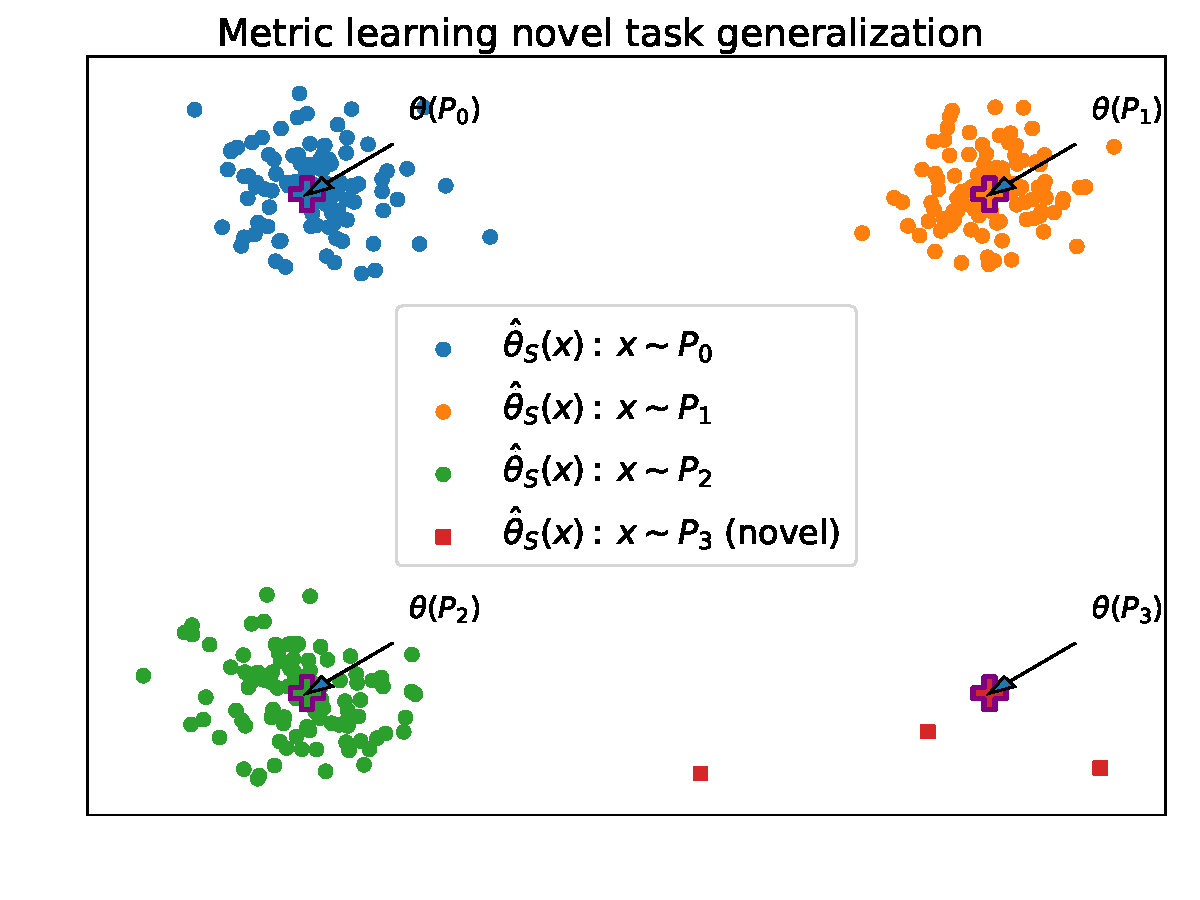
\includegraphics[width=\linewidth]{images/metric_learning_env.pdf}
%     % }
%     \caption{\textbf{Metric learning (synthetic):} An embedding function is estimated that is on-average close to a true representation of each task (`+'). The embeddings are shown compared to the target representation for each task distribution.}
%     \label{fig:metric_learning_env}
% \end{minipage}
% \begin{minipage}{\textwidth}
% \centering
% \fbox{
\iflatexml
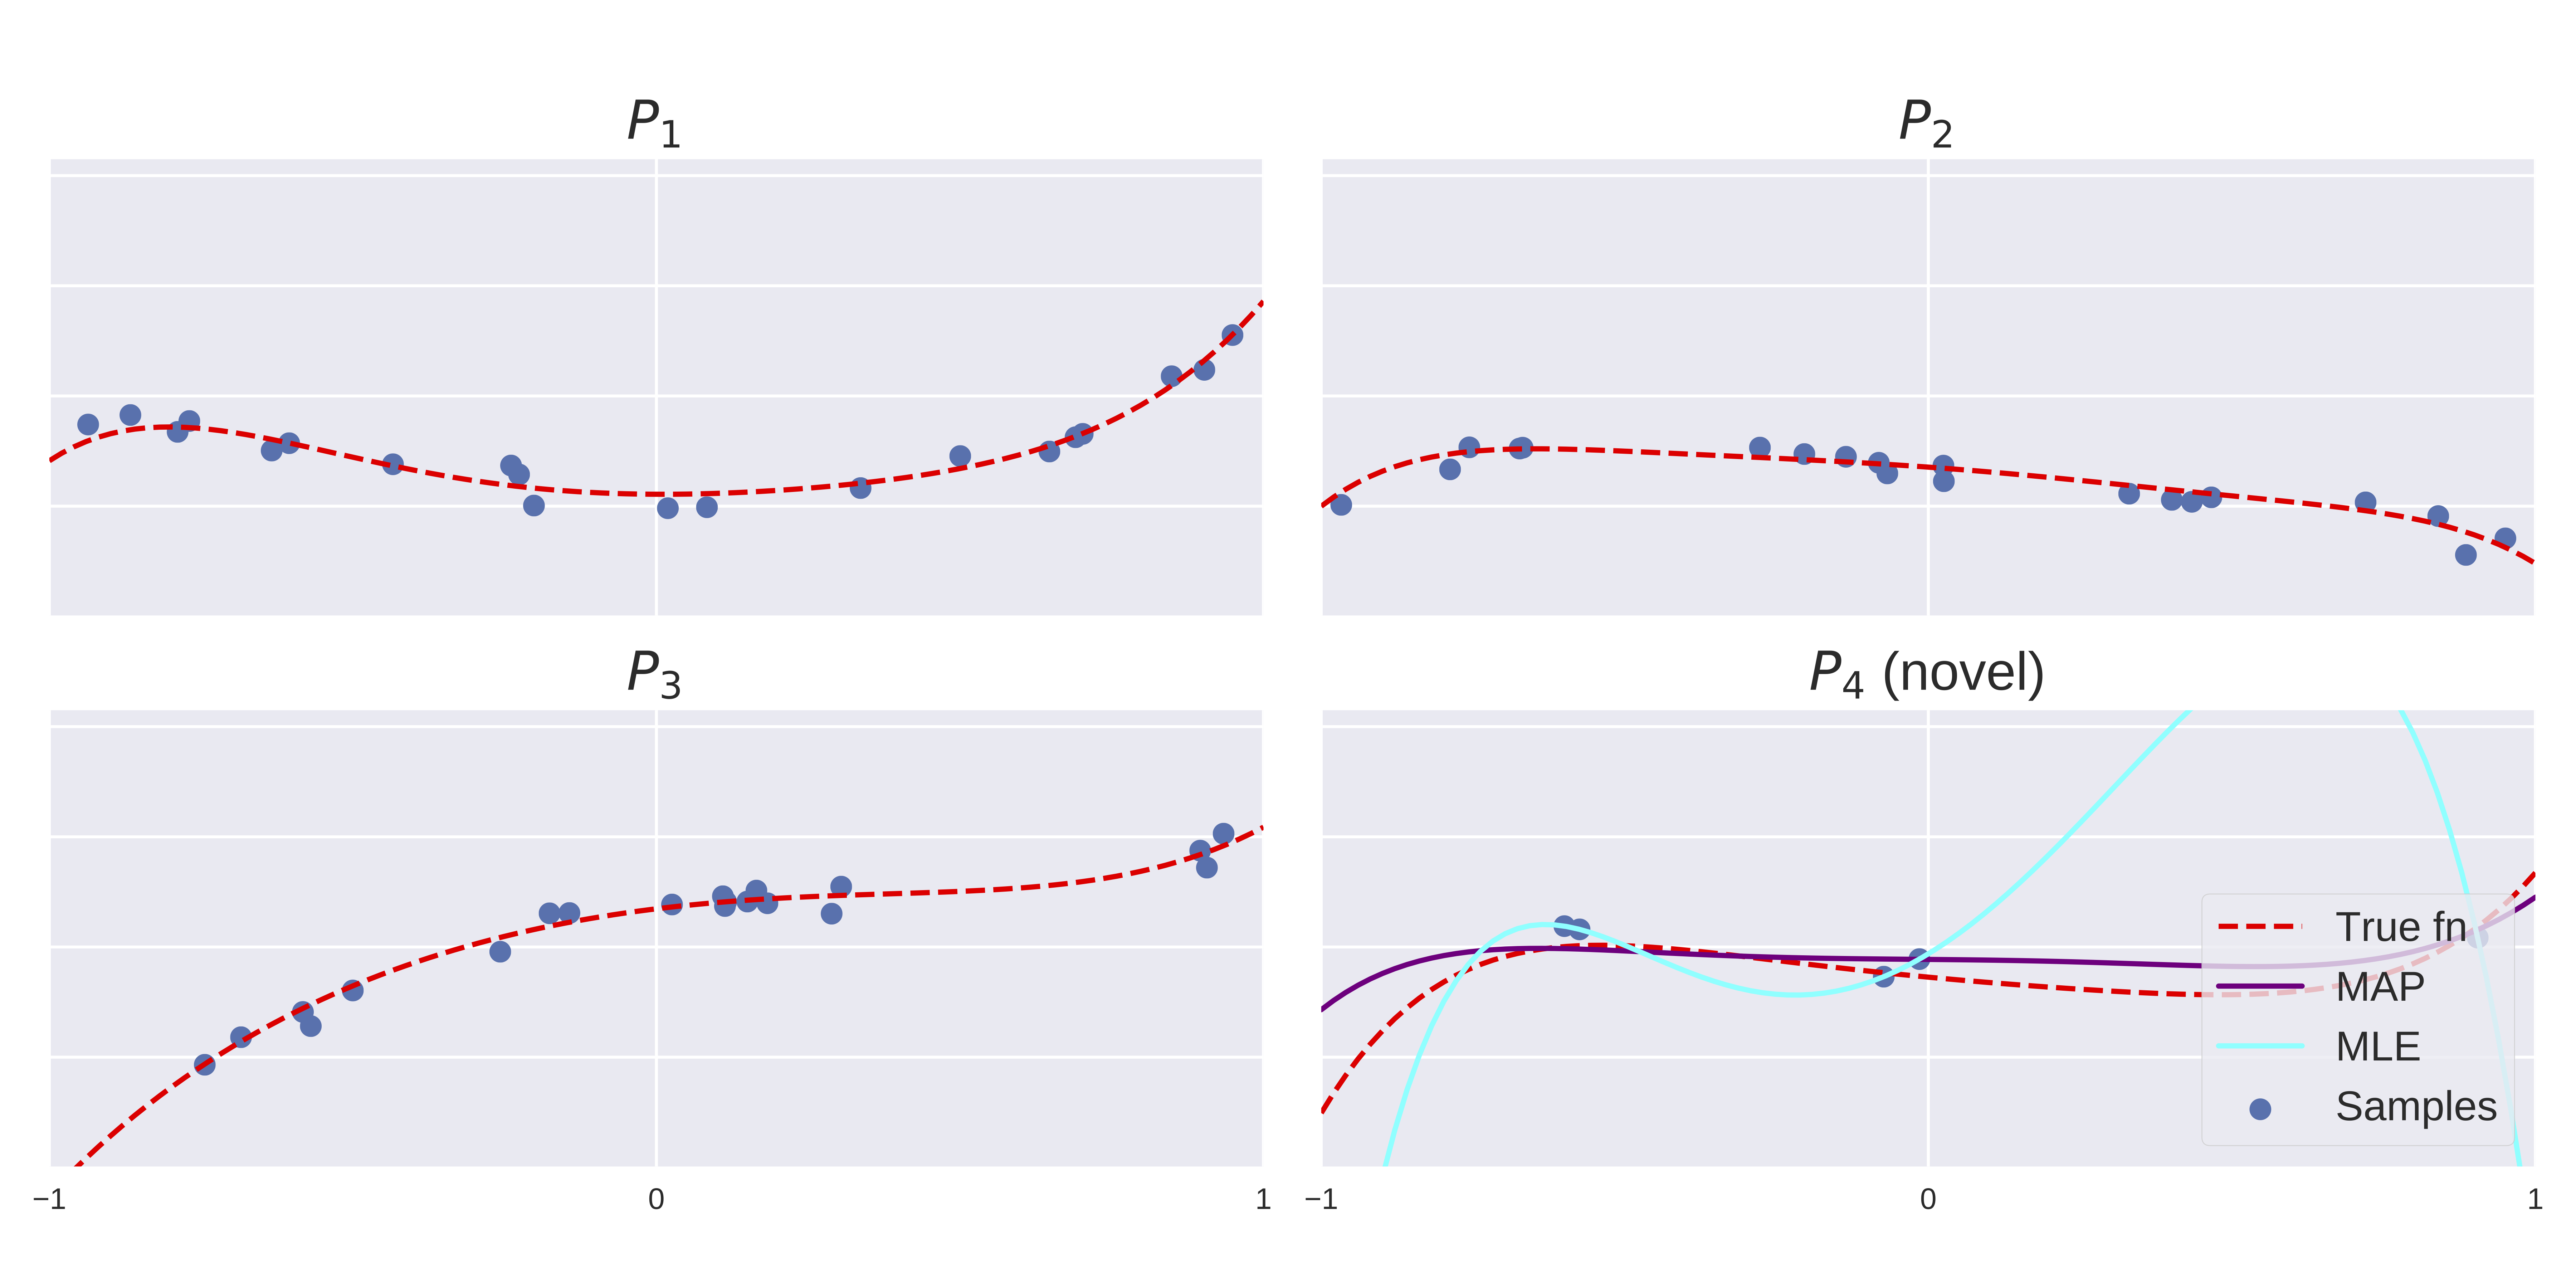
\includegraphics[width=6\linewidth]{main/images/meta_regression.png}%
\else
\centering
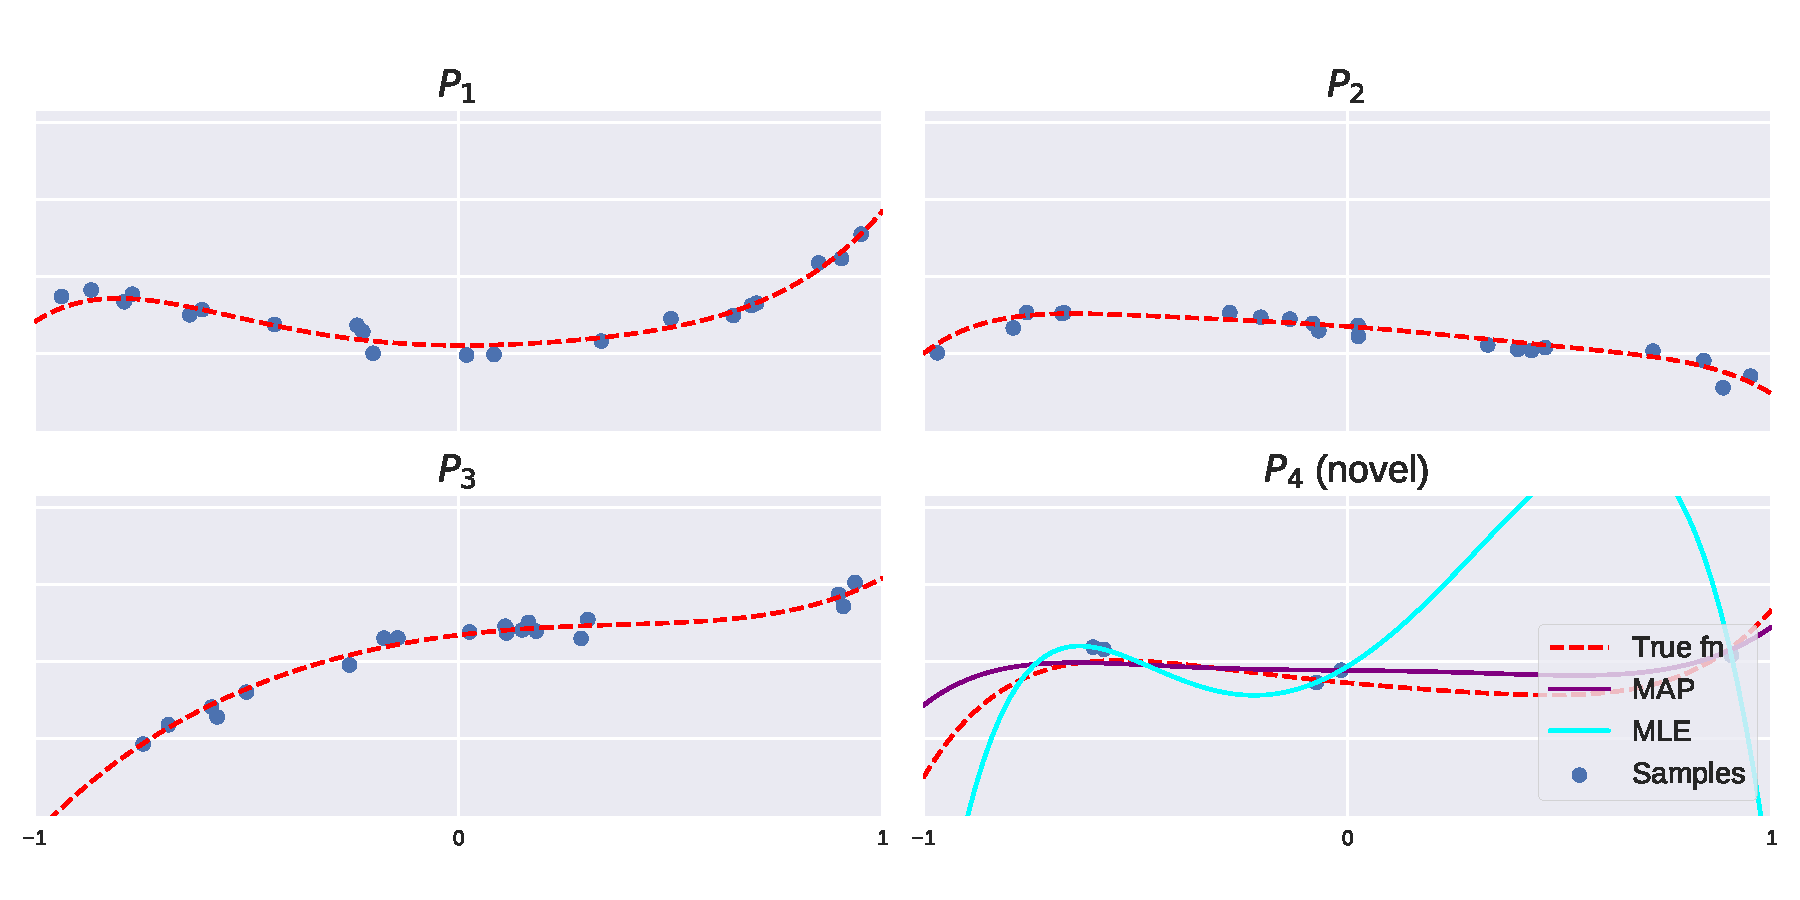
\includegraphics[width=\linewidth]{main/images/meta_regression.pdf}%
\fi
% }
\caption{\textbf{Meta-learning 1D-regression:} The parameters of a 1D regression model are fitted
from a small support set. The training distributions ($P_1,P_2,P_3$) give a useful inductive bias
for fitting $P_4$ using only 5 points. The MLE solution on the novel task for those 5 points is also
displayed.}
\label{fig:meta_lin_ref}
% \end{minipage}
\end{figure}
In Figure~\ref{fig:meta_lin_ref}, we show observed data samples from a family of polynomial
regression models. Our aim is to output an algorithm which recovers the parameters of a new polynomial function from limited observations--we choose a MAP estimator which is described fully in
Section~\ref{sec:hierarchical_bayes}. In the bottom right, we are given only 5 data points from a
novel task distribution and estimate the parameters of the model with both the MLE and MAP
estimators --- the MLE overfits the support set while the MAP estimator is close to the true function.

In terms of the terminology used above, the set,
\[\calP = \{p_{\lregparams}(y)=\calN(\bx^\top \lregparams,\sigma^2): \lregparams \in \bbR^{d}, \bx=[1,x,\ldots,x^{d-1}]\},\]
is the space of polynomial regression models, parameterized by $\lregparams$. For this problem, we take $\lossfn(\estimator, \theta) = \norm{\estimator - \theta}_2^2$. In Figure~\ref{fig:meta_lin_ref}, tasks are generated with $p(\theta) = \calN(\tau, \sigma^2_\theta)$, for unknown, sparse, $\tau \in \bbR^d$. Thus, each model is a polynomial function with few large coefficients. The algorithm $f$, first takes samples from $P_1,P_2,P_3$ and computes an estimate, $\hat{\tau}$. This estimate of $\tau$ is then used to compute $\bestimator(\testS; \hat{\tau}) = \argmax_{\lregparams_4} p(\lregparams_4|\hat{\tau}, \testS)$. Note that this approach is able to learn the correct inductive bias from the data, without requiring a carefully designed regularizer.  The lower bounds we derive in Section~4 can be applied to problems of this general type, and the upper and lower bounds in Section~5 apply specifically to meta-learning linear regression.